\section{Реализация метода}
\label{sec:Chapter5} \index{Chapter5}

% Перед тем как сформулировать постановку экспериментов и продемонстрировать результаты, аргументируется выбор Python в качестве языка программирования, а PyTorch в качестве фреймворка машинного обучения, для проведения экспериментов.

% \subsection{Выбор языка программирования}
% Выбор Python в качестве языка программирования для глубокого обучения
% Глубокое обучение стало одной из ключевых областей в искусственном интеллекте, и выбор языка программирования играет решающую роль в успехе проектов. Рассмотрим основные языки программирования, используемые в этой области, и обоснуем, почему Python является наиболее предпочтительным.

% \subsubsection{Python}
% Python является наиболее популярным языком для глубокого обучения благодаря своей простоте и широкому спектру библиотек, таких как TensorFlow, Keras и PyTorch. Простота синтаксиса Python позволяет сосредоточиться на алгоритмах и моделях, а не на технических деталях программирования. Кроме того, Python поддерживает объектно-ориентированное, процедурное и функциональное программирование, что делает его универсальным инструментом для различных задач глубокого обучения.

% \subsubsection{C++}
% C++ славится своей скоростью и эффективностью, что делает его хорошим выбором для систем, требующих высокой производительности, таких как роботы и автономные транспортные средства. Однако сложность синтаксиса и время, необходимое на разработку и отладку программ, делают C++ менее привлекательным для исследователей и разработчиков, сосредоточенных на быстром прототипировании и экспериментировании.

% \subsubsection{R}
% R был разработан специально для статистического анализа и визуализации данных, что делает его полезным инструментом для анализа данных и статистического моделирования. Однако для глубокого обучения R уступает Python в плане производительности и наличия специализированных библиотек. Кроме того, синтаксис R считается более сложным для изучения, чем у Python.

% \subsubsection{MATLAB}
% MATLAB предоставляет мощные инструменты для работы с матрицами и числовыми вычислениями, что важно для некоторых аспектов глубокого обучения. Однако его использование ограничено высокими затратами на лицензии и меньшим сообществом пользователей. В то время как MATLAB обладает высокопроизводительными встроенными функциями, Python с его бесплатными библиотеками часто оказывается более экономически эффективным и гибким решением.

% \subsubsection{Java}
% Java известен своей масштабируемостью и надежностью, что делает его подходящим для построения крупномасштабной инфраструктуры ИИ. Однако более сложный синтаксис и необходимость в большем объеме кода по сравнению с Python затрудняют быстрое прототипирование моделей глубокого обучения. Кроме того, экосистема библиотек для глубокого обучения в Java не столь развита, как у Python.

% \subsubsection{Сравнение и выбор}
% Несмотря на преимущества каждого из рассмотренных языков программирования, Python выделяется своей простотой, универсальностью и богатой экосистемой библиотек для глубокого обучения. Эти факторы делают его наиболее подходящим выбором как для начинающих, так и для опытных разработчиков в области глубокого обучения. Python позволяет эффективно разрабатывать, тестировать и внедрять модели глубокого обучения, что подтверждается его широким использованием в академической среде и промышленности.

% \subsection{Выбор фреймворка глубокого обучения}

% Для проведения научного исследования в глубоком обучении требуется мощные и гибкие инструменты для построения и обучения нейронных сетей. Помимо этого, такой фреймворк должен обеспечивать простоту реализации задач для того, чтобы процесс проведения экспериментов не занимал долгое время. Для решения этого вопроса рассмотрим наиболее популярные библиотеки.

% \subsubsection{TensorFlow}
% TensorFlow, разработанный Google, является одним из наиболее популярных фреймворков для глубокого обучения. Он поддерживает как символическое, так и императивное программирование, что позволяет пользователям выбирать между статическим и динамическим построением графов вычислений. TensorFlow широко используется в промышленности благодаря его высокой производительности и возможности развертывания на различных платформах, включая мобильные устройства и серверы.

% Основные преимущества TensorFlow:
% \begin{itemize}
%     \item поддержка распределенных вычислений;
%     \item интеграция с другими инструментами Google, такими как TensorBoard для визуализации и анализа проведенных экспериментов;
%     \item широкая библиотека предварительно обученных моделей.
% \end{itemize}

% Однако, TensorFlow обладает значительной сложностью, особенно для начинающих исследователей, и требует большего объема кода для простых операций.

% \subsubsection{Keras}
% Keras, первоначально разработанный как высокоуровневая библиотека поверх Theano и TensorFlow, стремится упростить разработку моделей глубокого обучения. Он предоставляет удобный и интуитивно понятный интерфейс для создания нейронных сетей.

% Основные преимущества Keras:
% \begin{itemize}
%     \item простота использования и быстрота прототипирования, что полезно для проведения научных исследований;
%     \item поддержка нескольких бэкендов, включая TensorFlow и Theano.
% \end{itemize}

% Тем не менее, ограниченные возможности по сравнению с низкоуровневыми фреймворками могут быть недостатком для сложных и специфических задач.

% \subsubsection{PyTorch}
% PyTorch, разработанный Facebook AI Research, представляет собой фреймворк для глубокого обучения, который стал популярным благодаря своей простоте и гибкости. PyTorch поддерживает динамическое построение графов вычислений, что делает его идеальным для научных исследований и экспериментов.

% Основные преимущества PyTorch:
% \begin{itemize}
%     \item интуитивно понятный и лаконичный синтаксис, напоминающий стандартный Python-код;
%     \item поддержка динамических вычислений, что упрощает отладку и экспериментирование с моделями;
%     \item широкая поддержка сообществом и наличие множества ресурсов для обучения и примеров.
% \end{itemize}

% \subsubsection{JAX}
% JAX, разработанный Google Research, представляет собой мощный инструмент для численных вычислений и машинного обучения, который сочетает в себе возможности библиотек Autograd и XLA. В данном обзоре рассмотрим особенности и преимущества JAX, а также его применение и отличия от PyTorch.

% JAX предлагает API, схожий с NumPy, но с возможностью выполнения вычислений на GPU и TPU, что значительно ускоряет процессы. Основные функции JAX включают:

% Преимущества JAX:
% \begin{itemize}
%     \item \textbf{производительность}: Благодаря компилятору XLA, JAX обеспечивает высокую производительность и оптимизацию вычислений на GPU и TPU;
%     \item гибкость: Позволяет исследователям легко экспериментировать с новыми архитекторами моделей и алгоритмами.
% \end{itemize}

% \subsubsection{Сравнение и выбор}
% Для научных экспериментов в области глубокого обучения ключевыми факторами являются простота использования, гибкость, поддержка сообществом и возможности для прототипирования. PyTorch выделяется среди других фреймворков благодаря:
% \begin{itemize}
%     \item интуитивно понятному и читаемому коду, что снижает порог вхождения для начинающих исследователей;
%     \item динамическому построению графов вычислений, что упрощает отладку и экспериментирование;
%     \item активному сообществу и большому количеству образовательных ресурсов, что способствует быстрому освоению и применению фреймворка.
% \end{itemize}

% Исходя из рассмотренных факторов, PyTorch является наиболее подходящим инструментом для научных экспериментов в сфере глубокого обучения. Его простота, гибкость и поддержка сообществом делают его идеальным выбором для исследователей, стремящихся к быстрому прототипированию и адаптации моделей. Несмотря на сильные стороны TensorFlow и других фреймворков, PyTorch обеспечивает оптимальный баланс между функциональностью и удобством использования, что критически важно в научной работе.

\subsection{Эксперименты}
Для эмпирического подтверждения факта, что данный метод решения задачи мостов Шрёдингера удовлетворяет поставленным требованиям, рассматриваются два эксперимента:
\begin{itemize}
    \item эксперимент на 2D данных;
    \item эксперимент на EMNIST.
\end{itemize}
Все эксперименты доступны в github репозитории\footnote{https://github.com/gregkseno/masters-thesis/tree/master}.

\subsubsection{2D данные}
Перед проверкой метода на данных большой размерности, проводится эксперимент на 2D данных, который предназначен, во-первых, для санитарного теста работоспособности метода, а, во-вторых, для проверки способности отображения при различных параметрах $\gamma$.

\begin{figure}
    \centering
    \subfloat[Кольца]{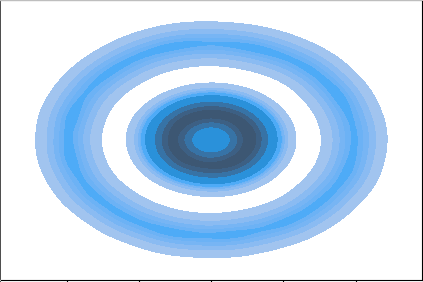
\includegraphics[width=0.4\linewidth]{images/circles.png}}
    \hfill
    \subfloat[Луны]{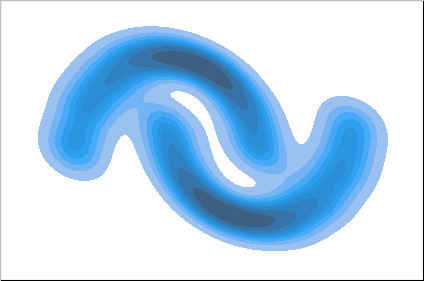
\includegraphics[width=0.4\linewidth]{images/moons.png}}   
    \subfloat[Рулет]{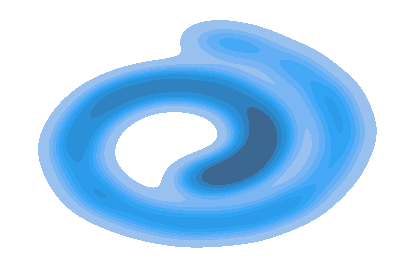
\includegraphics[width=0.4\linewidth]{images/swiss_roll.png}}   
    \caption{Набор 2D данных}
    \label{fig:moons-circles}
\end{figure}

Данными для 2D экспериментов послужили наборы из библиотеки sci-kit learn, а именно кольца, луны и рулет (рисунок \ref{fig:moons-circles}). Данные наборы представляют собой набор пар координат точек в плоскости.

Для санитарной проверки были выбраны кольца и луны в качестве $X$ и $Y$, соответственно. Для формирования набора лун были использованы следующие параметры:
\begin{itemize}
    \item количество точек обучающей выборки: $5000$;
    \item параметр стандартного отклонения шума, добавленного к данным: $0.05$
\end{itemize}

Для колец выбраны следующие параметры:
\begin{itemize}
    \item количество точек обучающей выборки: $5000$;
    \item параметр стандартного отклонения шума, добавленного к данным: $0.03$
    \item расстояние от между кольцами: $0.3$
\end{itemize}

Генератор параметризуется с помощью $3$-х полно-связных слоев. Каждый слой имеет $256$ нейронов. ReLU был выбран в качестве желаемой функции активации.

Для параметризации дискриминатора используется почти та же архитектура: $3$ полно-связных слоя со скрытыми слоем размером $256$, однако вместо ReLU, функцией активации является LeakyReLU с коэффициентом угла $0.2$. На вход подается конкатенация элементов из $X$ и $Y$, а на выходе скаляр. 

Также для лучшей сходимости после каждого линейного слоя генератора и дискриминатора применялась послойная нормализация.

Параметры оптимизаторов были выбраны следующие: 
\begin{itemize}
    \item используется AdamW в качестве алгоритма оптимизации;
    \item коэффициентом L2 регуляризации является значение $0,1$ для генератора и для дискриминатора;
    \item скорости обучения были установлены $1e-6$ для генераторов и дискриминаторов;
    \item размер батча был выбран $1024$
    \item модели обучались на протяжении $400$ эпох, а количество шагов состязательного обучения составило $60$;
    \item в качестве параметра $\gamma$ было выбрано значение $0.1$.
\end{itemize}

\begin{figure}
    \centering
    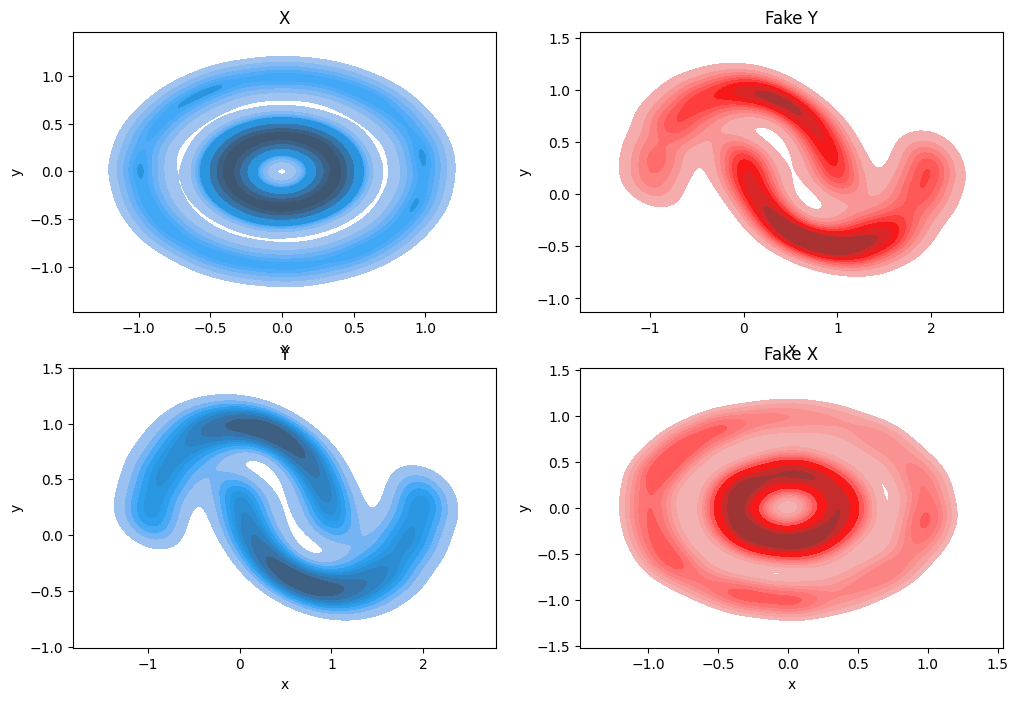
\includegraphics[width=1\linewidth]{images/2d_results.png}
    \caption{Результаты трансляции на кольцах, $X$, и  лунах, $Y$, с $\gamma = 0.1$}
    \label{fig:2d-res}
\end{figure}

Из результатов, изображенных на рисунке \ref{fig:2d-res}, понятно, что метод хорошо справляется с данными распределениями. Помимо визуального сходства, также можно заметить, что метод не сжимает или разжимает маргинальные распределения, таким образом сгенерированные элементы распределены с теми же средним и дисперсией.

Для сравнения трансляций при различных $\gamma$ 2D данных был выбраны стандартная гауссиана и рулет, для $X$ и $Y$, соответственно. Для рулета выбраны следующие параметры:
\begin{itemize}
    \item количество точек обучающей выборки: $5000$;
    \item параметр стандартного отклонения шума, добавленного к данным: $0.5$
\end{itemize}

\begin{figure}
    \centering
    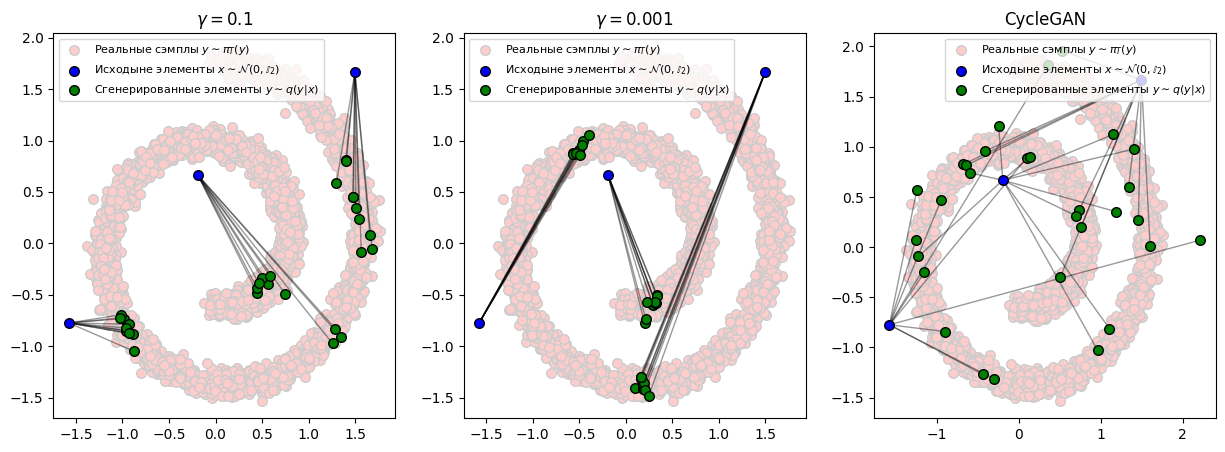
\includegraphics[width=1\linewidth]{images/2d_gamma.png}
    \caption{Сравнение трансляций точек предложенного метода с различными $\gamma$ и CycleGAN}
    \label{fig:2d-gamma}
\end{figure}

Целью данного эксперимента является анализ различия трансляций предложенного метода с различными $\gamma$ и CycleGAN \cite{cycle-gan}. Для этого эксперимента главным гиперпараметром является $\gamma$. В монографии \cite{monography-sbp} показано, что некоторые методы работают при больших $\gamma = 1000$, а некоторые — при низких $\gamma = 1$. Меньшее значение $\gamma$ гарантирует меньшее разброс отображенных элементов, то есть менее разнообразный вывод. В экскрементах были протестированы следующие параметры $\gamma$: $0.1$ и $0.001$.

Результаты (рисунок \ref{fig:2d-gamma}) демонстрируют, что метод отлично справляется с малыми параметрами $\gamma$. Также можно заметить, что при различных $\gamma$, действительно, отображение становится менее разнообразным. Более того, сравнивая предложенный метод с CycleGAN, транслированные элементы находятся в некоторой окрестности друг от друга, что не скажешь про трансляции CycleGAN.

\subsubsection{EMNIST}

\begin{figure}
    \centering
    \subfloat[Трансляция из букв в цифры]{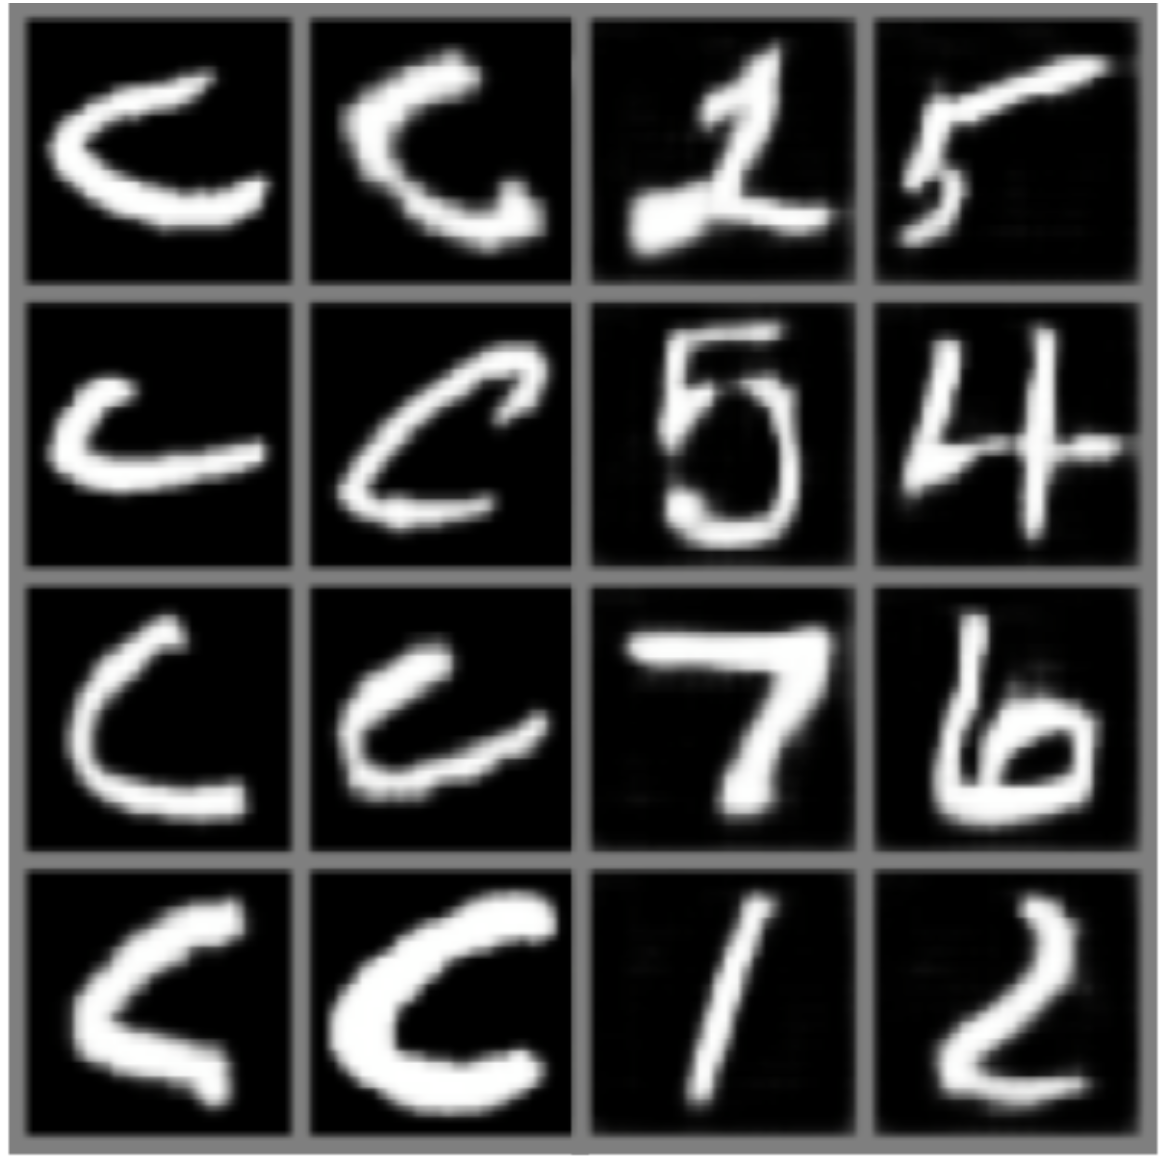
\includegraphics[width=0.4\linewidth]{images/emnist_cond_p.png}}
    \hfill
    \subfloat[Трансляция из цифр в буквы]{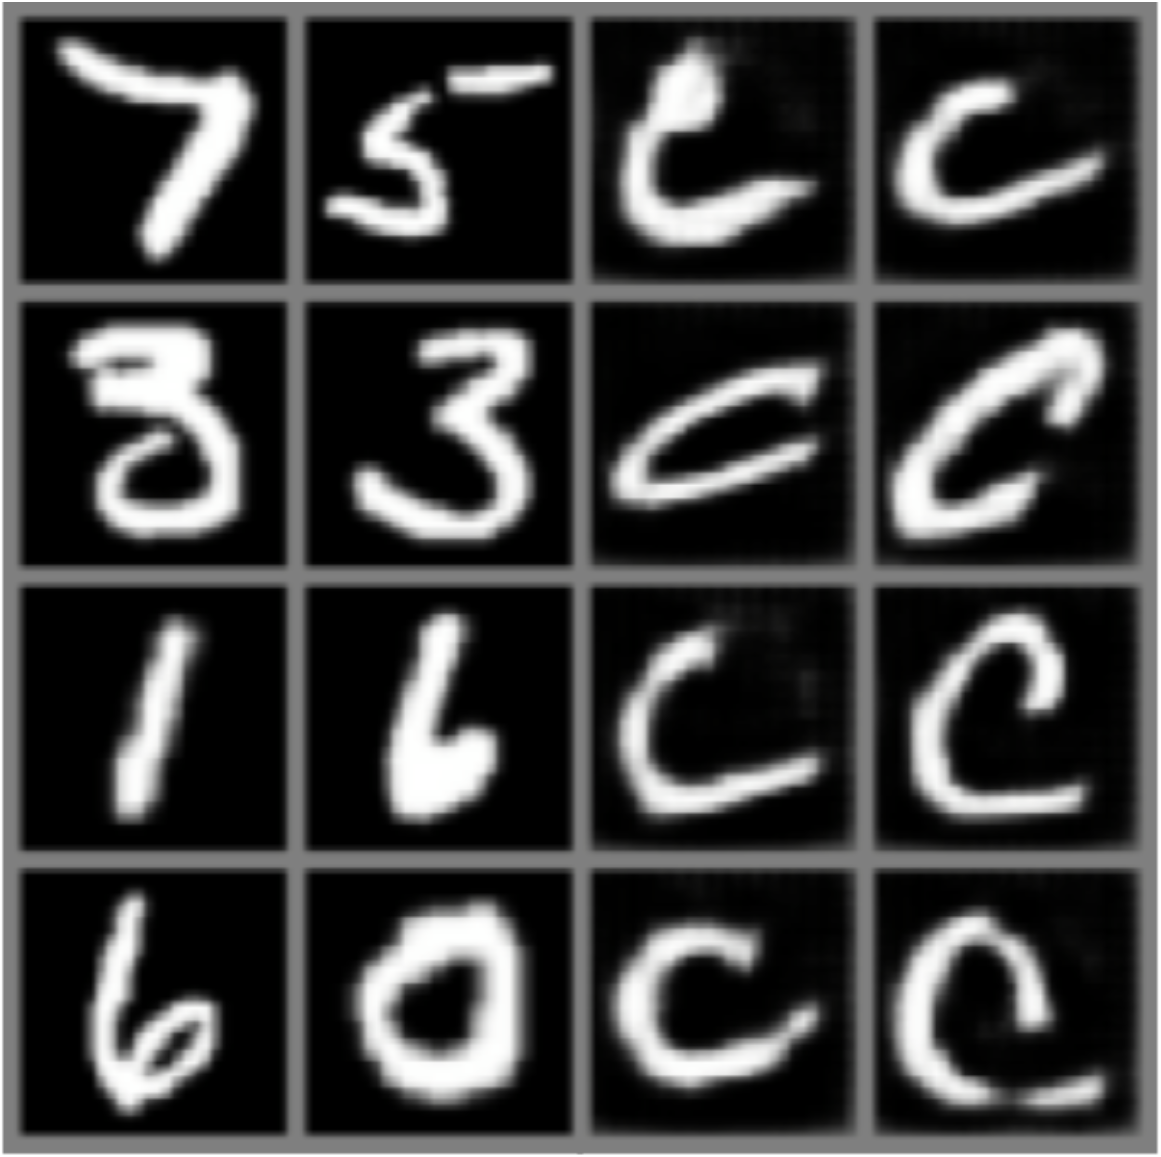
\includegraphics[width=0.4\linewidth]{images/emnist_cond_q.png}}  
    \caption{Пример трансляции на набор данных EMNIST}
    \label{fig:emnist-res}
\end{figure}

Целью данного эксперимента является подтверждение того факта, что метод работает на данных большой размерностью. Для этого был выбран набор данных EMNIST, который представляет собой набор рукописных символов, полученных из специальной базы данных NIST 19 и преобразованных в формат изображения 28x28 пикселей и структуру набора данных, которая напрямую соответствует набору данных MNIST.

В качестве набора $X$ был выбран поднабор EMNIST, а именно 145,600 латинских рукописных букв с 26 классами. В качестве $Y$ был выбран классический MNIST, в котором 70,000 цифр. Классы обоих наборов были сбалансированы. 

В качестве архитектуры генератора и дискриминатора для данного эксперимента использовались сверхточные слои с нормализацией по батчу, с вероятностью дропаута $0.2$, а также с функцией активации LeakyReLU с углом наклона $0.2$. Чтобы соответствовать области определения изображений $[0, 1]$, последней функцией генератора была выбрана гиперболический тангенс. Полную архитектуру можно посмотреть на рисунках \ref{fig:gen}, \ref{fig:disc}.

\begin{figure}
    \centering
    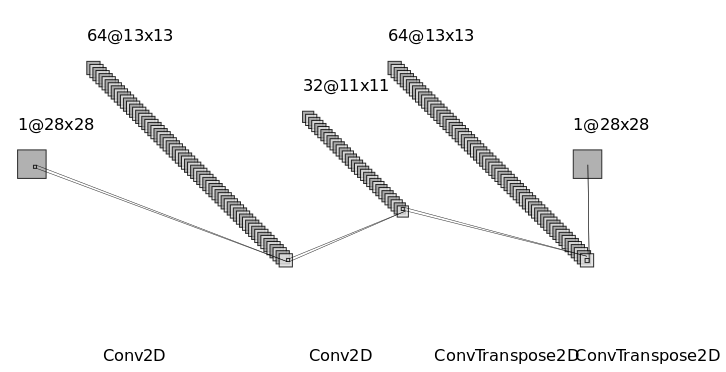
\includegraphics[width=0.8\linewidth]{images/generator.png}
    \caption{Архитектура генератора}
    \label{fig:gen}
\end{figure}

\begin{figure}
    \centering
    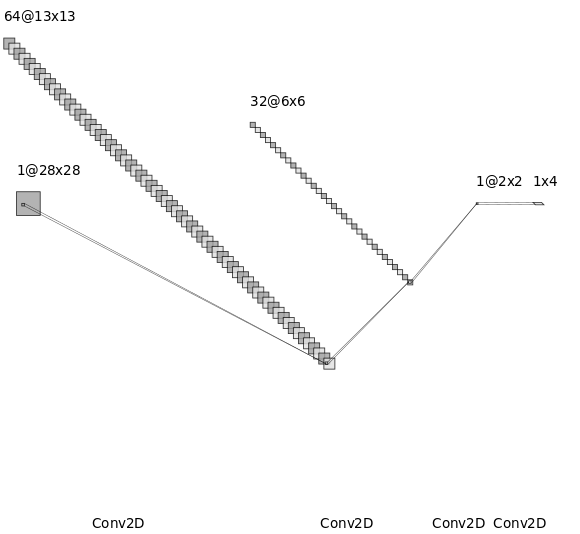
\includegraphics[width=0.6\linewidth]{images/disc.png}
    \caption{Архитектура дискриминатора}
    \label{fig:disc}
\end{figure}

Параметры оптимизаторов были выбраны следующие: 
\begin{itemize}
    \item используется AdamW в качестве алгоритма оптимизации;
    \item коэффициентом L2 регуляризации является значение $0,1$ для генератора и для дискриминатора;
    \item скорости обучения были установлены $1e-5$ для генераторов и дискриминаторов;
    \item размер батча был выбран $4096$
    \item модели обучались на протяжении $300$ эпох, а количество шагов состязательного обучения составило $60$;
    \item в качестве параметра $\gamma$ было выбрано значение $1$.
\end{itemize}

Результаты данного эксперимента продемонстрированы на рисунке \ref{fig:emnist-res}. Таким образом, можно заключить, что данный метод справляется с данными большой размерностью.

Также стоит отметить, что размерность 28x28 не является действительно большой и предыдущие методы, например Diffusion Schrödinger Bridge, также в качестве данных для экспериментов использовали EMNIST. Ожидается, что предложенный метод также можно использовать на данных большей размерностью, однако проведение таких экспериментов было не возможно в силу отсутствия вычислительных ресурсов.

\newpage
